\chapter{DreamDateの機能}
\label{chap:search}

この章ではDreamDateのシステムの概要と利用方法 について述べる。

\section{概要}
DreamDateは睡眠中にユーザの思い出と関連した音を流すことで、その音に関連した夢を見ることを促進するiOSスマートフォンアプリである。ターゲットのユーザは懐かしい思い出をもう一度体験したい人や、物理的に会えない人と会いたい人などである。DreamDateは開発途中でまだAppストアには掲示していないがgithubからソースコードを入手することが可能である。\\

\subsection{機能}
DreamDateには3つの機能がある。一つ目は寝る前に印象に残っている記憶に関する写真と映像を表示する機能。二つ目は睡眠中にレム睡眠を検出し記憶を連想させる音を流す機能。人は夢を見ている際に脳は記憶の整理をしているという研究結果があるため、被験者がかつて実際に体験したことと関連の高い音を利用する。例えば特別な誰かを連想する音、旅行中によく聞いていた曲、最寄り駅の音楽、好きな映画のサウンドトラックなどが適している。三つ目は起床後に夢について記録する夢日記機能である。ユーザには睡眠前にスマートフォンを画像\ref{DreamDateImage}のように枕の横に置いてもらう。\\
\begin{figure}[htbp]
\begin{center}
\includegraphics[width=11cm]{eps/dreamDate02.eps}
\caption{DreamDateの配置}
\label{DreamDateImage}
\end{center}
\end{figure}

\subsection{システム}
Xcode上でopenframeworksライブラリを利用したiPhoneの加速度センサーを利用した体動(寝返り)検知アプリケーションを制作した。図\ref{system}に一連のプログラムの流れを記載する。\\
\begin{figure}[htbp]
\begin{center}
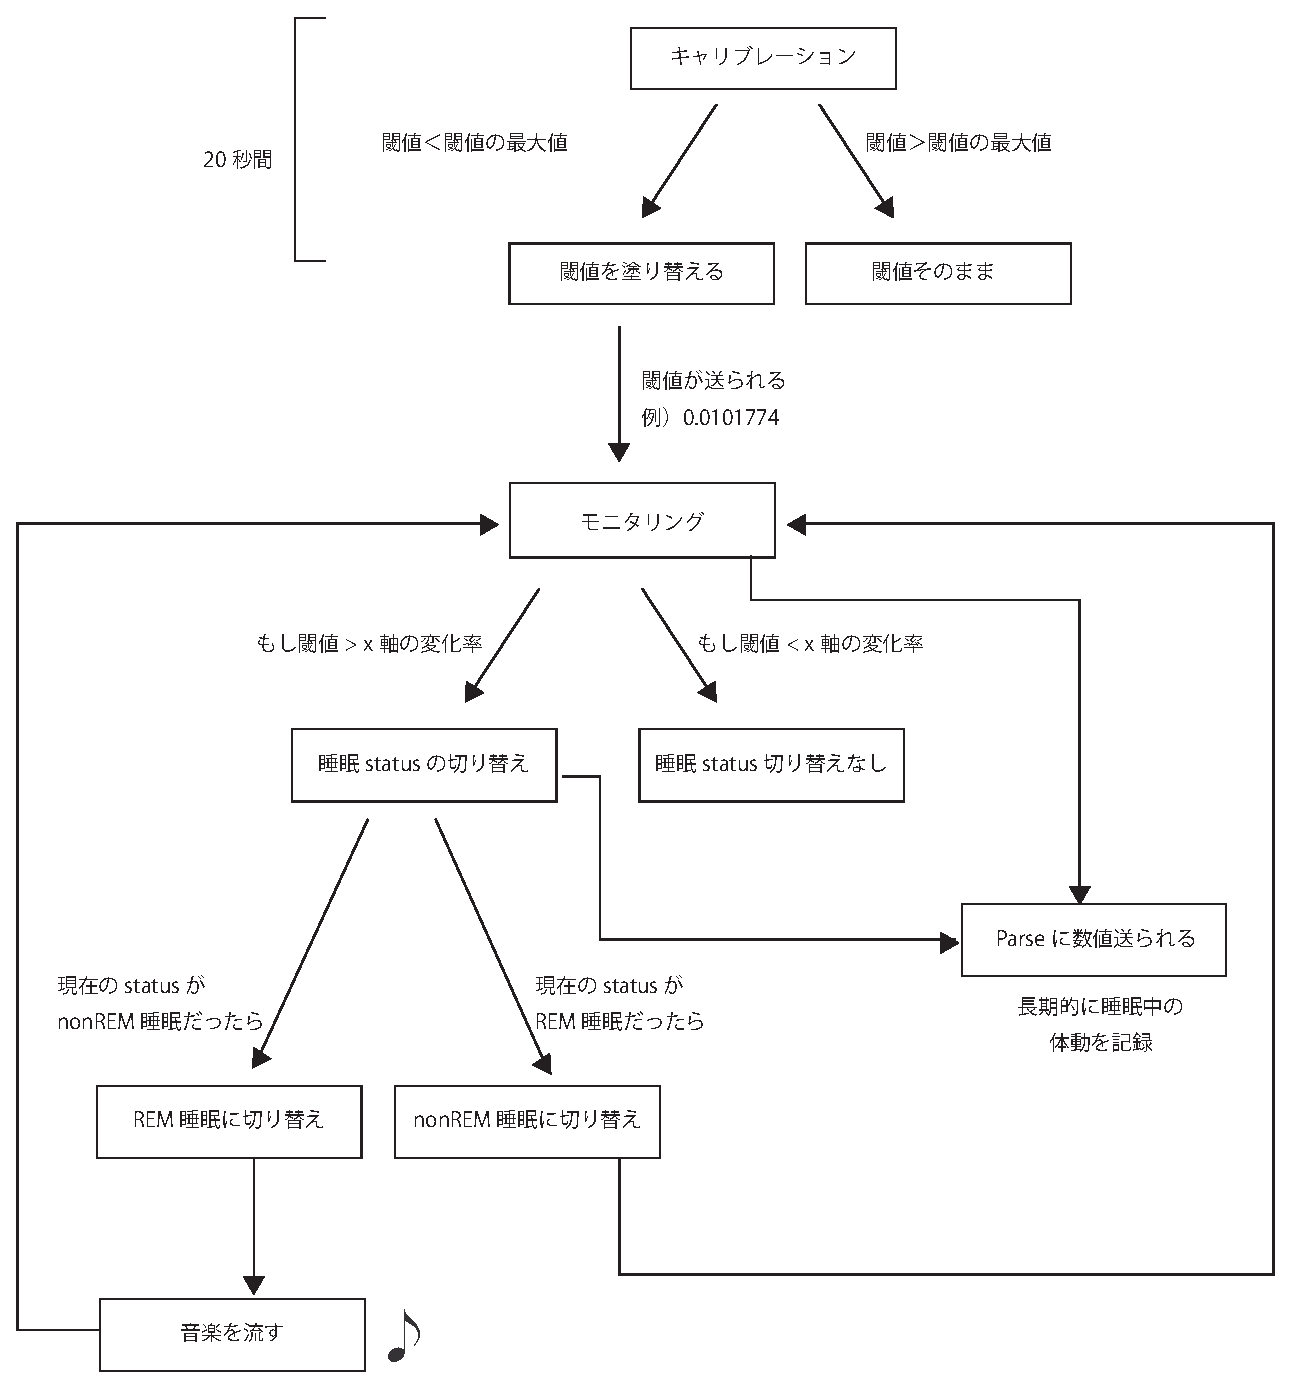
\includegraphics[width=15cm]{eps/system.eps}
\caption{DreamDateのフローチャート}
\label{system}
\end{center}
\end{figure}
ベッドの硬さは人により違うため、ユーザ自身にまずキャリブレーションをしてもらう。そのためにアプリ起動後ユーザにはiPhoneを横に置いた状態で15秒間静止してもらう。x軸の加速度を毎秒記録、1秒前の加速度との差分を導き出す。20秒間、x軸の差分の中での最大値を閾値として設定する。y軸とz軸の測定をしなかったのはx軸だけでも十分寝返りを特定できるためである。ベッドで寝てから睡眠に至るまで平均的に10分から20分かかるとされているため、スタートボタンが押されてから20分後に加速度センサーによる体動のモニタリングが開始される。こうすることで寝ようとしている最中に音楽がならないようにする。モニタリングの開始後はノイズを除去するために毎20秒の平均値が出される。その平均値が閾値に比べて高くなった時に寝返りをしたと判定する。寝返りを打つ時は睡眠段階がレム睡眠からノンレム睡眠に、あるいはノンレム睡眠からレム睡眠への切り替わったときとされているため\cite{negaeri}、図\ref{data_acceleration}は同じ日にDreamDateとiSleepそれぞれで観測した睡眠サイクルである。比べると大幅一致していることがわかる。図\ref{melodyGraph}で示したオレンジのタイミング(レム睡眠中)に登録しておいた音楽が流れる。レム睡眠時にのみ音楽を流すのは、常に音楽が流れていると睡眠が害され睡眠サイクルが崩れて体調不良などを引き起こす可能性が高くなるためである。一晩中のx軸の数値、音楽の再生状況、夢日記の結果はMBaaS(Mobile Backend as a Service)のサービスであるParseに保存する\cite{parse}。

\begin{figure}[htbp]
\begin{center}
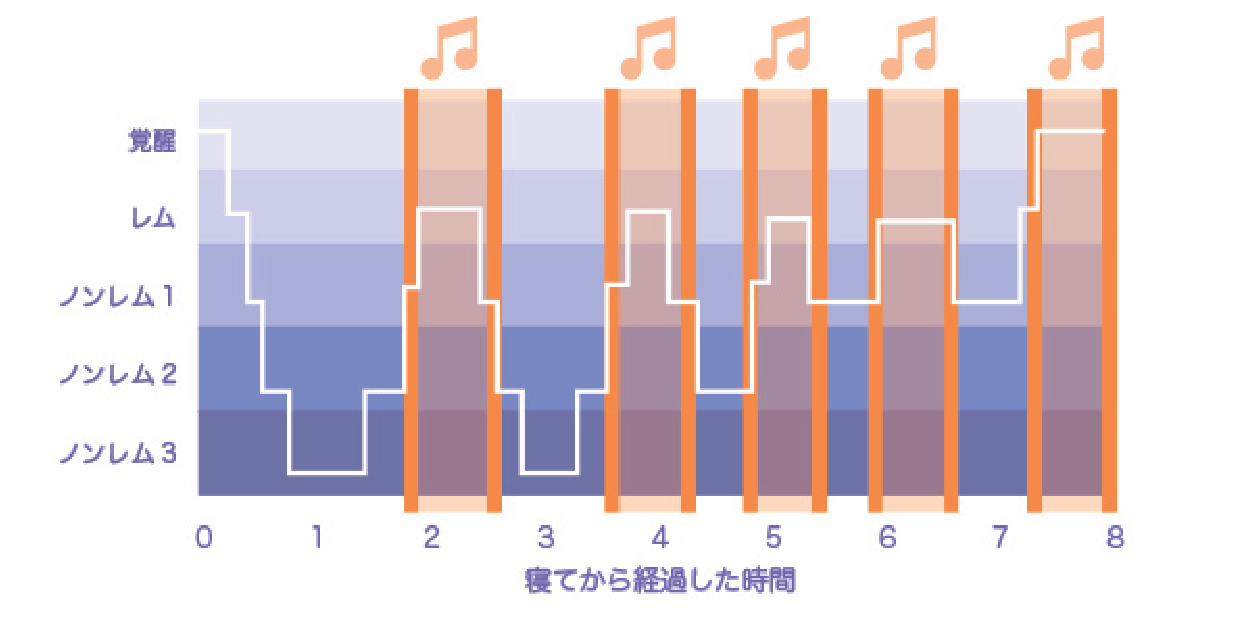
\includegraphics[width=13cm]{eps/remNonrem.eps}
\caption{音刺激提示のタイミング}
\label{melodyGraph}
\end{center}
\end{figure}

\begin{figure}[htbp]
\begin{center}
\includegraphics[width=15cm]{eps/data_acceleration.eps}
\caption{DreamDateで観測した睡眠サイクル }
\label{data_acceleration}
\end{center}
\end{figure}

\section{利用方法}
まずユーザには予め記憶を思い起こさせる音と画像を登録してもらう。音選びは適さない音があるため注意する必要がある。第4章でも述べるが、人の声を流すとユーザを起こしてしまう可能性が高いということが実験結果から分かった。特に喋りかけてくるような内容の音声は起こされやすい。その一方でレム睡眠中に流すのに適している音は繰り返しある環境下で聞いていた音である。アプリの起動後図\ref{le01}のような画面が表示される。そこには「自動ロック機能をOFFにする」「音量は1〜3に設定する」やiPhoneの置く位置などの指示が書かれている。次に図\ref{le02}の画面に遷移しユーザの思い出に関連性のある画像を表示する。ここでは寝る前に記憶の情景を思い出す機会を与えている。そして図\ref{le03}の画面では思い出の音楽が流れる。音楽を聴きながら、旅先での空間、香り、音の細部までを思い出して気持ちを落ちつかせて瞑想状態に入ってもらう。次に図\ref{le04}の画面に移動しユーザは実験日を選択する。実験日1は曲が流れない夜。実験日2はレム睡眠中ずっと曲が流れる。実験3は起きる前のレム睡眠のときのみ音が流れる。次に図\ref{le05}寝る前にアプリを起動してスタートボタンを押し、起動させたままスクリーンを伏せて枕の横に置く。20〜30分間後にDreamDateの体動検知が開始され、一晩中ユーザの体動のトラッキングが行われレム睡眠を検知すると音楽が鳴る。起床後図\ref{le06}の画面でユーザは起床すると夢の内容を忘れないように日記に投稿する。

\begin{figure}[htbp]
 \begin{minipage}{0.45\hsize}
  \begin{center}
   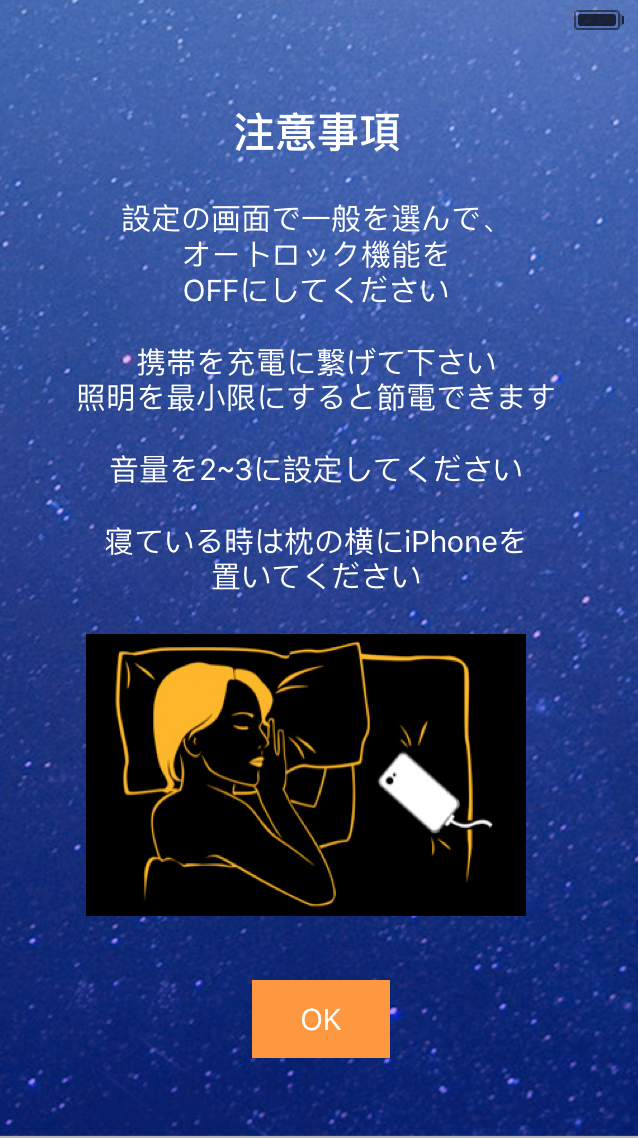
\includegraphics[height=90mm]{eps/AppIntro.eps}
  \end{center}
  \caption{起動画面}
  \label{le01}
 \end{minipage}
  \begin{minipage}{0.45\hsize}
  \begin{center}
   \includegraphics[height=90mm]{eps/AppMemoryImages.eps}
  \end{center}
  \caption{思い出の画像を表示}
  \label{le02}
 \end{minipage}
\end{figure}
\begin{figure}[htbp]
 \begin{minipage}{0.45\hsize}
  \begin{center}
   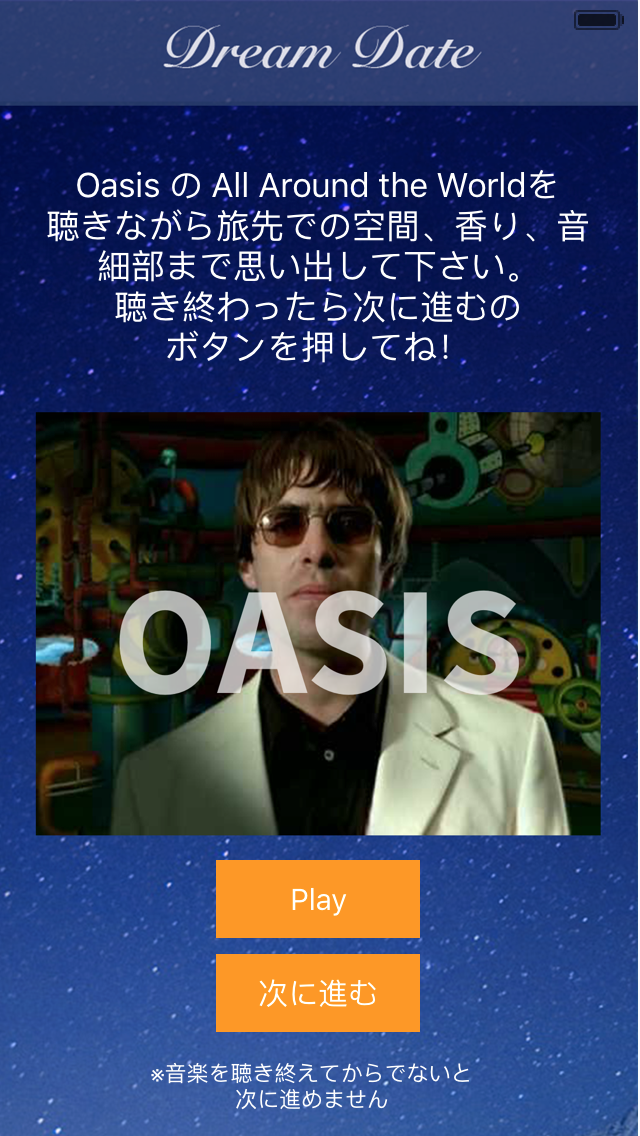
\includegraphics[height=90mm]{eps/AppMusicPlay.eps}
  \end{center}
  \caption{思い出に関連した音刺激の提示}
  \label{le03}
 \end{minipage}
 \begin{minipage}{0.45\hsize}
  \begin{center}
   \includegraphics[height=90mm]{eps/AppExperienmentType.eps}
  \end{center}
  \caption{実験日選択ボタン}
  \label{le04}
 \end{minipage}
\end{figure}

\begin{figure}[htbp]
 \begin{minipage}{0.45\hsize}
  \begin{center}
   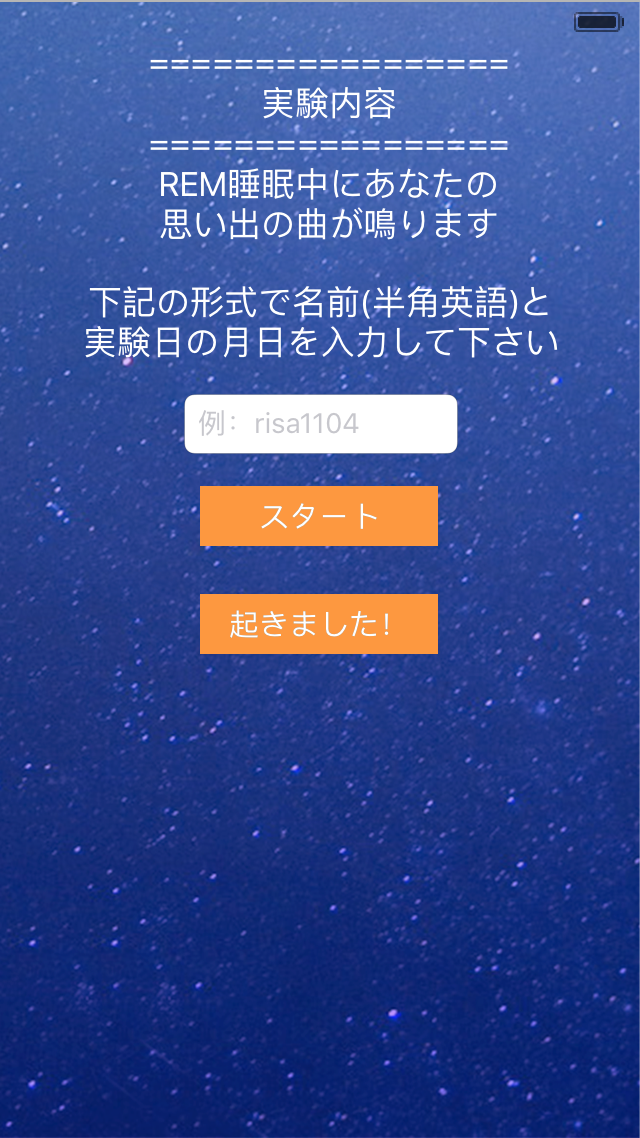
\includegraphics[height=90mm]{eps/AppStart.eps}
  \end{center}
  \caption{睡眠開始ボタン}
  \label{le05}
 \end{minipage}
 \begin{minipage}{0.45\hsize}
  \begin{center}
   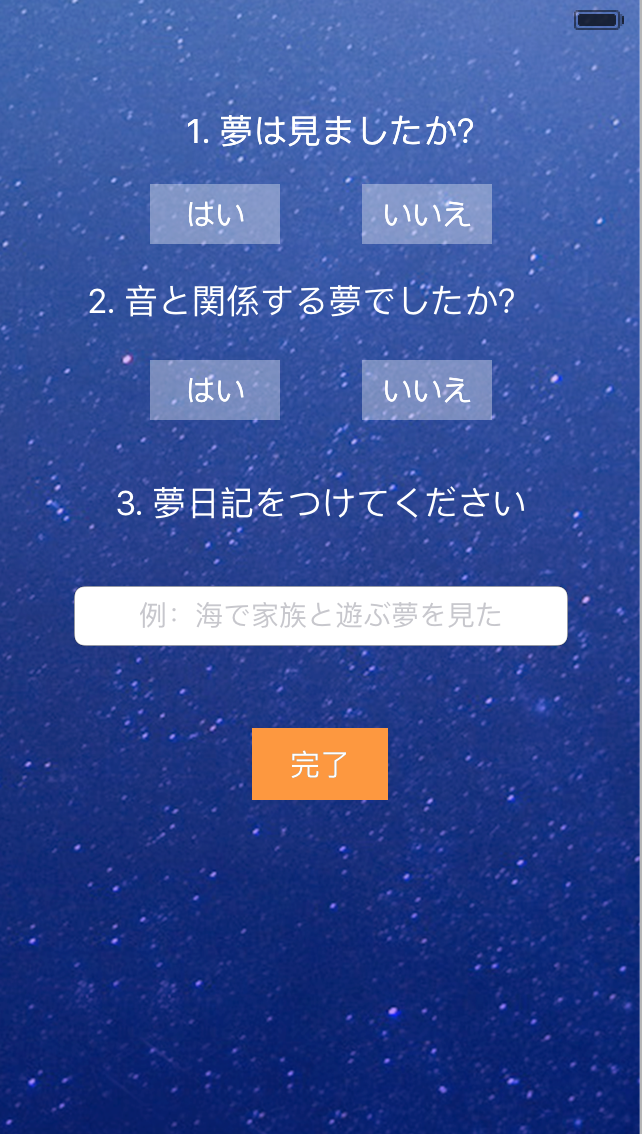
\includegraphics[height=90mm]{eps/AppDiary.eps}
  \end{center}
  \caption{夢日記記入ページ}
  \label{le06}
 \end{minipage}
\end{figure}